\begin{figure}
\centering

		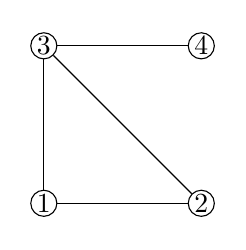
\begin{tikzpicture}
		\tikzset{tinoeud/.style={draw, circle, minimum height=0.1cm}}
		\node[tinoeud] (U) at (0,0) {};
		\node[tinoeud] (V) at (2,0) {};
		\node[tinoeud] (W) at (0,2) {};
		\node[tinoeud] (T) at (2,2) {};

    \draw (U) -- (V);
    \draw (V) -- (W);
    \draw (W) -- (U);
    \draw (W) -- (T);

    \draw (U) node {$1$};
    \draw (V) node {$2$};
    \draw (W) node {$3$};
    \draw (T) node {$4$};

		\end{tikzpicture}

		\begin{tikzpicture}
		
		\coordinate (O) at (0,0);

    \prgrid{O}{22}{22}

    \prvtline{O}{6}{22}
    \prvtline{O}{10}{22}
    \prvtline{O}{14}{22}
    \prvtline{O}{18}{22}
    
    \prvtcolumn{O}{6}{22}
    \prvtcolumn{O}{10}{22}
    \prvtcolumn{O}{14}{22}
    \prvtcolumn{O}{18}{22}
    
    \prvtdline{O}{7}{22}
    \prvtdline{O}{11}{22}
    \prvtdline{O}{15}{22}
    \prvtdline{O}{19}{22}
    
    \prvtdcolumn{O}{7}{22}
    \prvtdcolumn{O}{11}{22}
    \prvtdcolumn{O}{15}{22}
    \prvtdcolumn{O}{19}{22}
    
    \draw ($(O)+(-0.5,4)$) node {$v_1$};
    \draw ($(O)+(-0.5,6)$) node {$v_2$};
    \draw ($(O)+(-0.5,8)$) node {$v_3$};
    \draw ($(O)+(-0.5,10)$) node {$v_4$};
    
    \draw ($(O)+(4,-0.5)$) node {$v_1$};
    \draw ($(O)+(6,-0.5)$) node {$v_2$};
    \draw ($(O)+(8,-0.5)$) node {$v_3$};
    \draw ($(O)+(10,-0.5)$) node {$v_4$};

    \prone{O}{1}{1};
    \prone{O}{1}{2};
    \prone{O}{1}{3};
    \prone{O}{1}{4};
    \prone{O}{1}{5};
    \prone{O}{1}{6};
    
    \prone{O}{2}{1};
    \prone{O}{3}{1};
    \prone{O}{4}{1};
    \prone{O}{5}{1};
    \prone{O}{6}{1};
 
    \prone{O}{7}{1};
    \prone{O}{8}{3};
    \prone{O}{9}{3};
    \prone{O}{9}{5};
    \prone{O}{10}{5};
    \prone{O}{10}{1};
 
    \prone{O}{11}{1};
    \prone{O}{12}{3};
    \prone{O}{13}{3};
    \prone{O}{13}{5};
    \prone{O}{14}{5};
    \prone{O}{14}{1};
 
    \prone{O}{15}{1};
    \prone{O}{16}{3};
    \prone{O}{17}{3};
    \prone{O}{17}{5};
    \prone{O}{18}{5};
    \prone{O}{18}{1};
 
    \prone{O}{19}{1};
    \prone{O}{20}{3};
    \prone{O}{21}{3};
    \prone{O}{21}{5};
    \prone{O}{22}{5};
    \prone{O}{22}{1};
		
 
    \prone{O}{1}{7};
    \prone{O}{3}{8};
    \prone{O}{3}{9};
    \prone{O}{5}{9};
    \prone{O}{5}{10};
    \prone{O}{1}{10};
 
    \prone{O}{1}{11};
    \prone{O}{3}{12};
    \prone{O}{3}{13};
    \prone{O}{5}{13};
    \prone{O}{5}{14};
    \prone{O}{1}{14};
 
    \prone{O}{1}{15};
    \prone{O}{3}{16};
    \prone{O}{3}{17};
    \prone{O}{5}{17};
    \prone{O}{5}{18};
    \prone{O}{1}{18};
 
    \prone{O}{1}{19};
    \prone{O}{3}{20};
    \prone{O}{3}{21};
    \prone{O}{5}{21};
    \prone{O}{5}{22};
    \prone{O}{1}{22};


    \prone{O}{7}{7};
    \prone{O}{9}{9};

    \prone{O}{11}{11};
    \prone{O}{13}{13};

    \prone{O}{15}{15};
    \prone{O}{17}{17};

    \prone{O}{19}{19};
    \prone{O}{21}{21};


    \prone{O}{7}{19};
    \prone{O}{8}{20};

    \prone{O}{19}{7};
    \prone{O}{20}{8};

    \prone{O}{11}{19};
    \prone{O}{12}{20};

    \prone{O}{19}{11};
    \prone{O}{20}{12};

  
    \end{tikzpicture}

\caption{This figure illustrates, on the first part, a graph in which we search for a maximum clique and, on the second part, the matrix obtained built with the reduction. We do not show the 0 entries of the matrix for readability. }
\label{fig:reduction:example}
\end{figure}